\documentclass[12pt]{article}
% \usepackage{polski}
% \def\PLdateending{\space r.}

\title{J\\Słownik Lindego t. II s. 221}
\author{Janusz S. Bień (red.)}

\date{\today}
https://www.overleaf.com/2412909zxgyxs#
%%%%%%%%%%%%%%%%%%%%%%%%%%%%%%%%%%%%%%%%%%%%%%%%%%%%%%%

\usepackage{fontspec}

%\setmainfont{TeXGyreTermes}
%\setsansfont{TeXGyreTermes}
%\setmainfont{TeXGyreTermes}
%\setmainfont{DejaVu Serif}
%\setmainfont{Bitstream Vera Serif}

% double oblique hyphen:
\setmainfont{Linux Libertine O}
%\setmainfont{Courier New}

%\setmonofont{TeXGyreCursor}
\setmonofont{DejaVu Sans Mono}

% no math
\catcode`\&=12



\usepackage{graphicx}

\usepackage{hyperref}

\usepackage[para]{footmisc}

%%%%%%%%%%%%%%%%%%%%%%%%%%%%%%%%%%%%%%%%%%%%%%%%%%%%%%%

% LaTeX Companion 2nd ed., p. 127
\newcommand{\marginlabel}[1]{\mbox{}\marginpar{\raggedright\hspace{0pt}#1}}

%%%%%%%%%%%%%%%%%%%%%%%%%%%%%%%%%%%%%%%%%%%%%%%%%%%%%%%

\newcommand{\abbrev}[2]{#2}

\newcommand{\entry}[2]{#2}
\newcommand{\entryref}[2]{#2}

% double oblique hyphen
\newcommand{\doh}[1]{⸗}

% http://unifraktur.sourceforge.net/
% UnifrakturMaguntia
\newcommand{\fraktur}[1]{#1}

\newcommand{\gram}[1]{#1}

\newcommand{\mainentry}[2]{#2}
% 1 klasyfikacja hasła
% 2 
\newcommand{\mainentrybegin}[2]{\section{#2}}
% #1 prefiks lub jego brak
% #2 oryginalna pisownia hasła wersalikami
\newcommand{\mainentryend}[1]{}
% #1 oryginalna pisownia hasła wersalikami (powtórzona dla redundacji)
% komenda kończy wcięcie tekstu hasła

\newcommand{\mainentrypageend}[1]{}
% kontynuacja hasła na następnej stronie

\newcommand{\pos}[2]{#2}

\newcommand{\showimage}[1]{\includegraphics[width=1.0\textwidth]{img/#1}}

\newcommand{\quoteref}[1]{#1}

\newcommand{\subentry}[2]{#2}

\newcommand{\wikiq}[2]{\textit{#2}}


\begin{document}
\maketitle

\obeylines

\url{http://teksty.klf.uw.edu.pl/26/3/LindeIIGP+2i.djvu?djvuopts=&page=227&zoom=width&showposition=0.5,0.64&highlight=2140,3357,131,193}

\bigskip
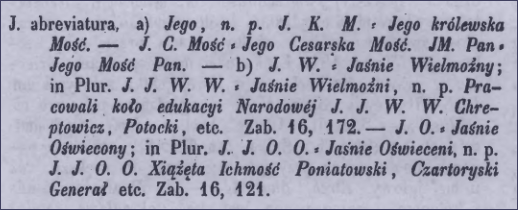
\includegraphics{J-Linde}

\smallskip
\noindent
J. abreviatura,

\begin{description}
\item[a)] \textit{Jego},
\textit{n. p.}
\textit{J. K. M.}  \doh{} \textit{Jego królewska Mość}.
---
\textit{J. C. Mość} ⸗ \textit{Jego Cesarska Mość}.
\textit{JM. Pan} ⸗ \textit{Jego Mość Pan}.
---
\item[b)] [Jaśnie]
\textit{J. W.} ⸗ \textit{Jaśnie Wielmożny};
in Plur. \textit{J. J. W. W.} ⸗ \textit{Jaśnie Wielmożni}
n. p.
\begin{quote}
\textit{Pracowali koło edukacyi Narodowéj J. J. W. W. Chreptowicz, Potocki,%
  etc.}
  Zab. 46, 472.
\end{quote}
---
\textit{J. O.} ⸗ \textit{Jaśnie Oświecony};
\textit{J. J. O. O}. ⸗ \textit{Jaśnie Oświeceni},
n.p.
\begin{quote}
  \textit{J. J. O. O. Xiążęta Ichmość Poniatowski, Czartoryski Generał etc.}
  Zab. 16, 121.
\end{quote}
\end{description}

\end{document}

#NAME "J 6"

{{Janusz S. Bień}}

{{blue: łacina}}

J

 [url]http://teksty.klf.uw.edu.pl/26/3/LindeIIGP+2i.djvu?djvuopts=&page=227&zoom=width&showposition=0.5,0.64&highlight=2140,3357,131,193[/url]

 [s]J-Linde.png[/s]

 J. abreviatura,
 [m1]a) [i]Jego[/i],[/m1]
 [m2][p]n. p.[/p][/m2]
 [m3][i]J. K. M. ⸗ Jego królewska Mość.[/i] — [/m3]
 [m3][i]J. C. Mość ⸗ Jego Cesarska Mość.[/i][/m3]
 [m3][i]JM. Pan ⸗ Jego Mość Pan.[/i] —[m3]
 [m1]b) \[Jaśnie\][/m1]
 [m2][i]J. W. ⸗ Jaśnie Wielmożny[/i]; [c blue]in [p]Plur.[/p][/c] [i]J. J. W. W. ⸗ Jaśnie Wielmożni[/i],[/m2]
 [m3][p]n. p.[/p][/m3]
 [m4][i]Pracowali kolo edukacyi Narodowej J. J. W. W.. Chreptowicz, Potocki,[/i] [p]etc.[/p] [p]Zab. 46, 472.[/p] — [i][m4]
 [m2][i]J. O. ⸗ Jaśnie Oświecony[/i]; [c blue]in [p]Plur.[/p][/c] [i]J. J. 0. 0. ⸗ Jasnie Oświeceni[/i],[/m2]
 [m3][p]n. p.[/p][/m3]
 [m4][i]J. J. O. O. Xiążęta Ichmość Poniatowski, Czartoryski Generał[/i] [p]etc.[/p] [p]Zab. 16, 121.[/p][m4]

 [m1][p]JSB[/p][m1]

{{
J. abreviatura., a) Jego, n. p. J. K. M. - Jego królewska
Mość. - J. 0. Mość - Jego Cesarska Mość. JM. Pan-
Jego Mość Pan. - b) J. W. - Jaśnie Wielmożny;
in Plur. J. J. W. W. - Jas'm'e Wielmożna', n. p. Pra-
cowali` kolo edukacyi Narodówe'j' J. J. W. W.. Chre-
ptowicz, Potocki, etc. Zab. 46, 472.- J. 0.sJaśnie
Oświecony; in" Plur. J.. J. 0. 0. - Jasnie Oświeceni, n. p.
J. J. -0. O. Xiąźęta Ichmość Poniatowski, Czartoryski
Generał etc. Zab. 16, 121.
}}
%%% Local Variables:
%%% mode: latex
%%% TeX-master: t
%%% TeX-engine: xetex
%%% End:
